%----------------------------------------------------------------------------------------
%	LATEX LABBOOK TEMPLATE
%	Versie 1.0 (12 september 2013)
%	Opmerkingen of feedback naar Robert van Wijk 
%					(robertvanwijk@uva.nl)
%----------------------------------------------------------------------------------------

%----------------------------------------------------------------------------------------
%	PACKAGES EN DOCUMENT CONFIGURATIE
%----------------------------------------------------------------------------------------

\documentclass[a4paper,12pt]{article}
\usepackage{graphicx}
\usepackage[dutch]{babel}
\usepackage{fancyhdr}
\usepackage{lastpage}
\usepackage{xifthen}
\usepackage{algorithm2e}
\usepackage{lipsum}
\usepackage{hyperref}
\usepackage{listings}
\usepackage{xcolor}
\lstset { %
    language=C++,
    backgroundcolor=\color{black!5}, % set backgroundcolor
    basicstyle=\footnotesize,% basic font setting
}

%----------------------------------------------------------------------------------------
%	HEADER & FOOTER
%----------------------------------------------------------------------------------------
\pagestyle{fancy}
  \lhead{
\includegraphics[width=7cm]{logoUvA}}		%Zorg dat het logo in dezelfde map staat
  \rhead{\footnotesize \textsc {Technisch rapport\\ \opdracht}}
  \lfoot
    {
	\footnotesize \studentA
	\ifthenelse{\isundefined{\studentB}}{}{\\ \studentB}
	\ifthenelse{\isundefined{\studentC}}{}{\\ \studentC}
	\ifthenelse{\isundefined{\studentD}}{}{\\ \studentD}
	\ifthenelse{\isundefined{\studentE}}{}{\\ \studentE}
    }
  \cfoot{}
  \rfoot{\small \textsc {Pagina \thepage\ van \pageref{LastPage}}}
  \renewcommand{\footrulewidth}{0.5pt}

\fancypagestyle{firststyle}
 {
  \fancyhf{}
   \renewcommand{\headrulewidth}{0pt}
   \chead{
\includegraphics[width=7cm]{logoUvA}}
   \rfoot{\small \textsc {Pagina \thepage\ van \pageref{LastPage}}}
 }

\setlength{\topmargin}{-0.3in}
\setlength{\textheight}{630pt}
\setlength{\headsep}{40pt}

%----------------------------------------------------------------------------------------
%	DOCUMENT INFORMATIE
%----------------------------------------------------------------------------------------
%Geef bij ieder command het juiste argument voor deze opdracht. Vul het hier in en het komt op meerdere plekken in het document correct te staan.

\newcommand{\titel}{Servo systeem bestuurd door Android apparaat}			%Zelfbedachte titel
\newcommand{\opdracht}{Mobile Systems Basic Design}		%Naam van opdracht die je van docent gehad hebt
\newcommand{\docent}{drs. A. van Inge}
\newcommand{\cursus}{Netcentric Computing}
\newcommand{\vakcode}{5062NECO6Y}		%Te vinden op oa Datanose
\newcommand{\datum}{\today}					%Pas aan als je niet de datum van vanaag wilt hebben
\newcommand{\studentA}{Shahrukh Zaidi}
\newcommand{\uvanetidA}{10636102}
\newcommand{\studentB}{Sjoerd Wenker}			%Comment de regel als je allen werkt
\newcommand{\uvanetidB}{10617558}
%\newcommand{\studentC}{Naam student 3}		%Uncomment de regel als je met drie studenten werkt
\newcommand{\uvanetidC}{UvAnetID student 3}
%\newcommand{\studentD}{Naam student 4}		%Uncomment de regel als je met vier studenten werkt
\newcommand{\uvanetidD}{UvAnetID student 4}
%\newcommand{\studentE}{Naam student 5}			%Uncomment de regel als je met vijf studenten werkt
\newcommand{\uvanetidE}{UvAnetID student 5}

%----------------------------------------------------------------------------------------
%	AUTOMATISCHE TITEL
%----------------------------------------------------------------------------------------
\begin{document}
\thispagestyle{firststyle}
\begin{center}
	\textsc{\Large \opdracht}\\[0.2cm]
		\rule{\linewidth}{0.5pt} \\[0.4cm]
			{ \huge \bfseries \titel}
		\rule{\linewidth}{0.5pt} \\[0.2cm]
	{\large \datum  \\[0.4cm]}
	
	\begin{minipage}{0.4\textwidth}
		\begin{flushleft} 
			\emph{Student:}\\
			{\studentA \\ {\small \uvanetidA \\[0.2cm]}}
				\ifthenelse{\isundefined{\studentB}}{}{\studentB \\ {\small \uvanetidB \\[0.2cm]}}
				\ifthenelse{\isundefined{\studentC}}{}{\studentC \\ {\small \uvanetidC \\[0.2cm]}}
				\ifthenelse{\isundefined{\studentD}}{}{\studentD \\ {\small \uvanetidD \\[0.2cm]}}
				\ifthenelse{\isundefined{\studentE}}{}{\studentE \\ {\small \uvanetidE \\[0.2cm]}}
		\end{flushleft}
	\end{minipage}
~
	\begin{minipage}{0.4\textwidth}
		\begin{flushright} 
			\emph{Docent:} \\
			\docent \\[0.2cm]
			\emph{Cursus:} \\
			\cursus \\[0.2cm]
			\emph{Vakcode:} \\
			\vakcode \\[0.2cm]
		\end{flushright}
	\end{minipage}\\[1 cm]
\end{center}

%----------------------------------------------------------------------------------------
%	INHOUDSOPGAVE EN ABSTRACT 
%----------------------------------------------------------------------------------------

%\tableofcontents
%\begin{abstract}
%\lorem[13]
%\end{abstract}

%----------------------------------------------------------------------------------------
%	INTRODUCTIE
%----------------------------------------------------------------------------------------
\section{Introductie}
In deze opdracht gaan wij een systeem bouwen dat het mogelijk maakt om een servosysteem door middel van een Android apparaat aan te sturen. Het servosysteem bestaat uit een elektromotor met op de as een potentiometer. Deze potentiometer wordt gebruikt om de aspositie van de servo op te meten. Om het servosysteem via een Android apparaat te be\"{i}nvloeden, wordt gebruik gemaakt van een mBed microcontroller. Deze staat direct aangesloten op de servo en kan onder andere worden gebruikt om de servomotor aan te sturen. Om uiteindelijk de servomotor met een Android toestel aan te sturen, wordt een toestel aangesloten op de mBed. De Android apparaten waarvan wij gebruik hebben gemaakt om het regelsysteem te testen, draaien op de nieuwste versie van Android (Android 6.0).  

\subsection{Opstelling}
De opstelling bestaat uit 4 componenten: het servosysteem, de mBed microcontroller en twee Android telefoons. In figuur \ref{fig:opstelling} is de opstelling te bezichtigen.
\vspace{1em}
\begin{figure}[!htbp]
\centering
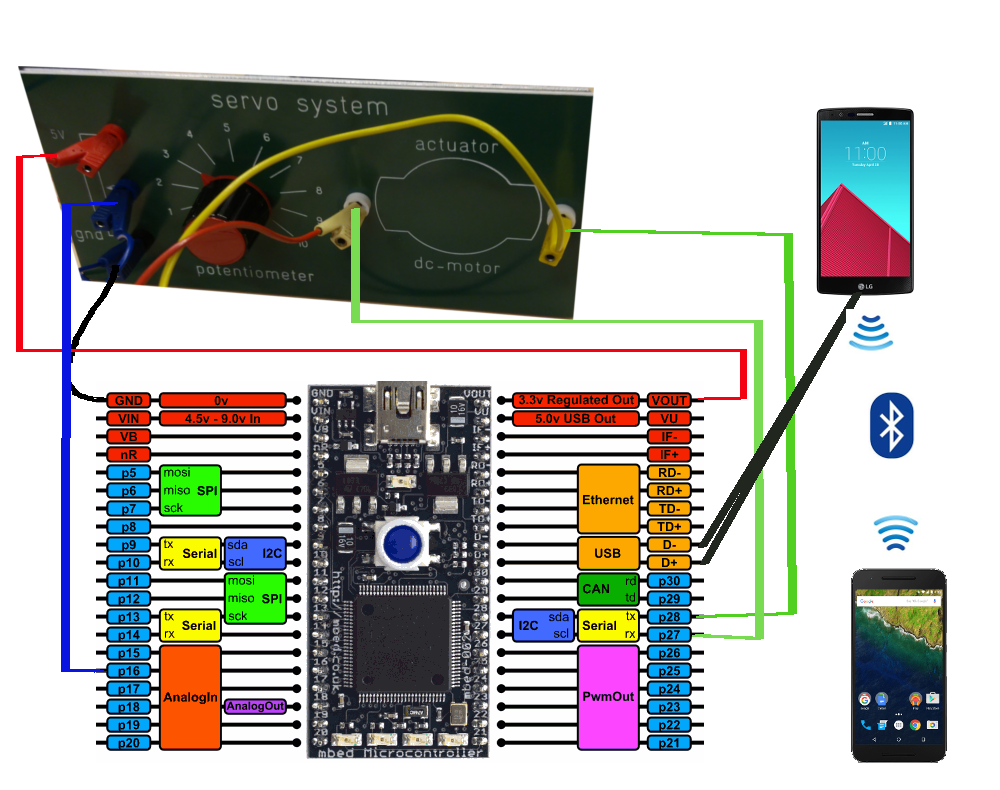
\includegraphics[width=0.5\textwidth, scale=0.5]{opstelling.png}
\vspace{1ex}
\hrule
\caption{Opstelling}
\label{fig:opstelling}
\end{figure}

In figuur \ref{fig:blokdiagram} is het blokdiagram van de opdracht te zien. De servo wordt bediend door de mBed controller. De waarde van de potentiometer verandert als de servo draait. Deze waarde kan uitgelezen worden door de mBed. Er is communicatie tussen de mBed controller en de slave Android telefoon. Hierdoor kan de slave commando's sturen naar de mBed controller. De slave kan bediend worden door een master Android telefoon door middel van een Bluetooth-verbinding.

\vspace{1em}
\begin{figure}[!htbp]
\centering
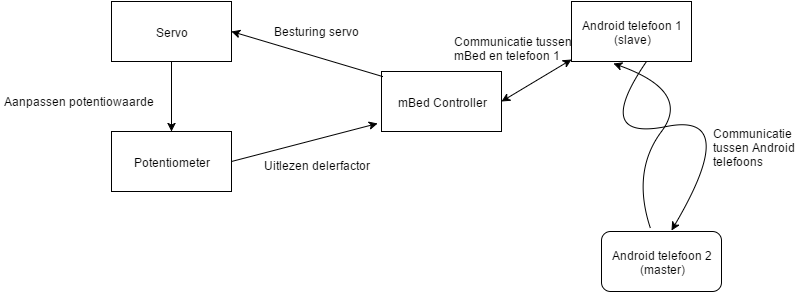
\includegraphics[width=1.2\textwidth]{blokdiagram.png}
\vspace{1ex}
\hrule
\caption{Opstelling}
\label{fig:blokdiagram}
\end{figure}

%----------------------------------------------------------------------------------------
%	METHODE
%----------------------------------------------------------------------------------------

\section{Methode}

\subsection{mBed-servo koppeling}
Het aansluiten van het servosysteem op de mBed microcontroller bestaat uit twee delen. Als eerste wordt de asopnemer aangesloten op de mBed. Hiervoor hebben wij gebruik gemaakt van de ADC pin \textit{p16}. Deze geeft, met behulp van de \texttt{read()}-functie de delerfactor (in dit verslag ook wel spanningsmeting genoemd) terug. Dit is een waarde tussen de 0 en 1 waarmee uiteindelijk de potentiowaarde kan worden berekend. Deze potentiowaarde ligt tussen de 0 en 10. De elektrische aardaansluiting wordt aangesloten op de GND-poort \textit{p22}. Voor het aansturen van de servomotor om de weerstand aan te passen, maken wij gebruik van de H-Bridge stroomversterker poorten \textit{p27} en \textit{p28}. In tabel \ref{tab:measurings} is te zien wat onze metingen waren bij de bijbehorende potentiowaarden.

\begin{table}[h!]
\centering
\label{tab:measurings}
\begin{tabular}{l | l}
Potentiowaarde & Gemeten gemiddelde delerfactor waarde \\
\hline
0              & 0.0000                               \\
0.5            & 0.001                                \\
1              & 0.0035                               \\
1.5            & 0.0075                               \\
2              & 0.015                                \\
2.5            & 0.0295                               \\
3              & 0.0455                               \\
3.5            & 0.0705                               \\
4              & 0.093                                \\
4.5            & 0.120                                \\
5              & 0.1435                               \\
5.5            & 0.168                                \\
6              & 0.1935                               \\
6.5            & 0.2235                               \\
7              & 0.260                                \\
7.5            & 0.3105                               \\
8              & 0.4335                               \\
8.5            & 0.566                                \\
9              & 0.7025                               \\
9.5            & 0.8135                               \\
10             & 0.964                                
\end{tabular}
\caption{Gemeten gemiddelde delerfactor waarden van potentiometer}
\end{table}

Om de huidige potentiowaarde te bepalen, hebben wij voor elke positie van de sensor, met een interval van een half, de gemeten spanning genoteerd. Dit levert de volgende grafiek op:

\vspace{1em}
\begin{figure}[!htbp]
\centering
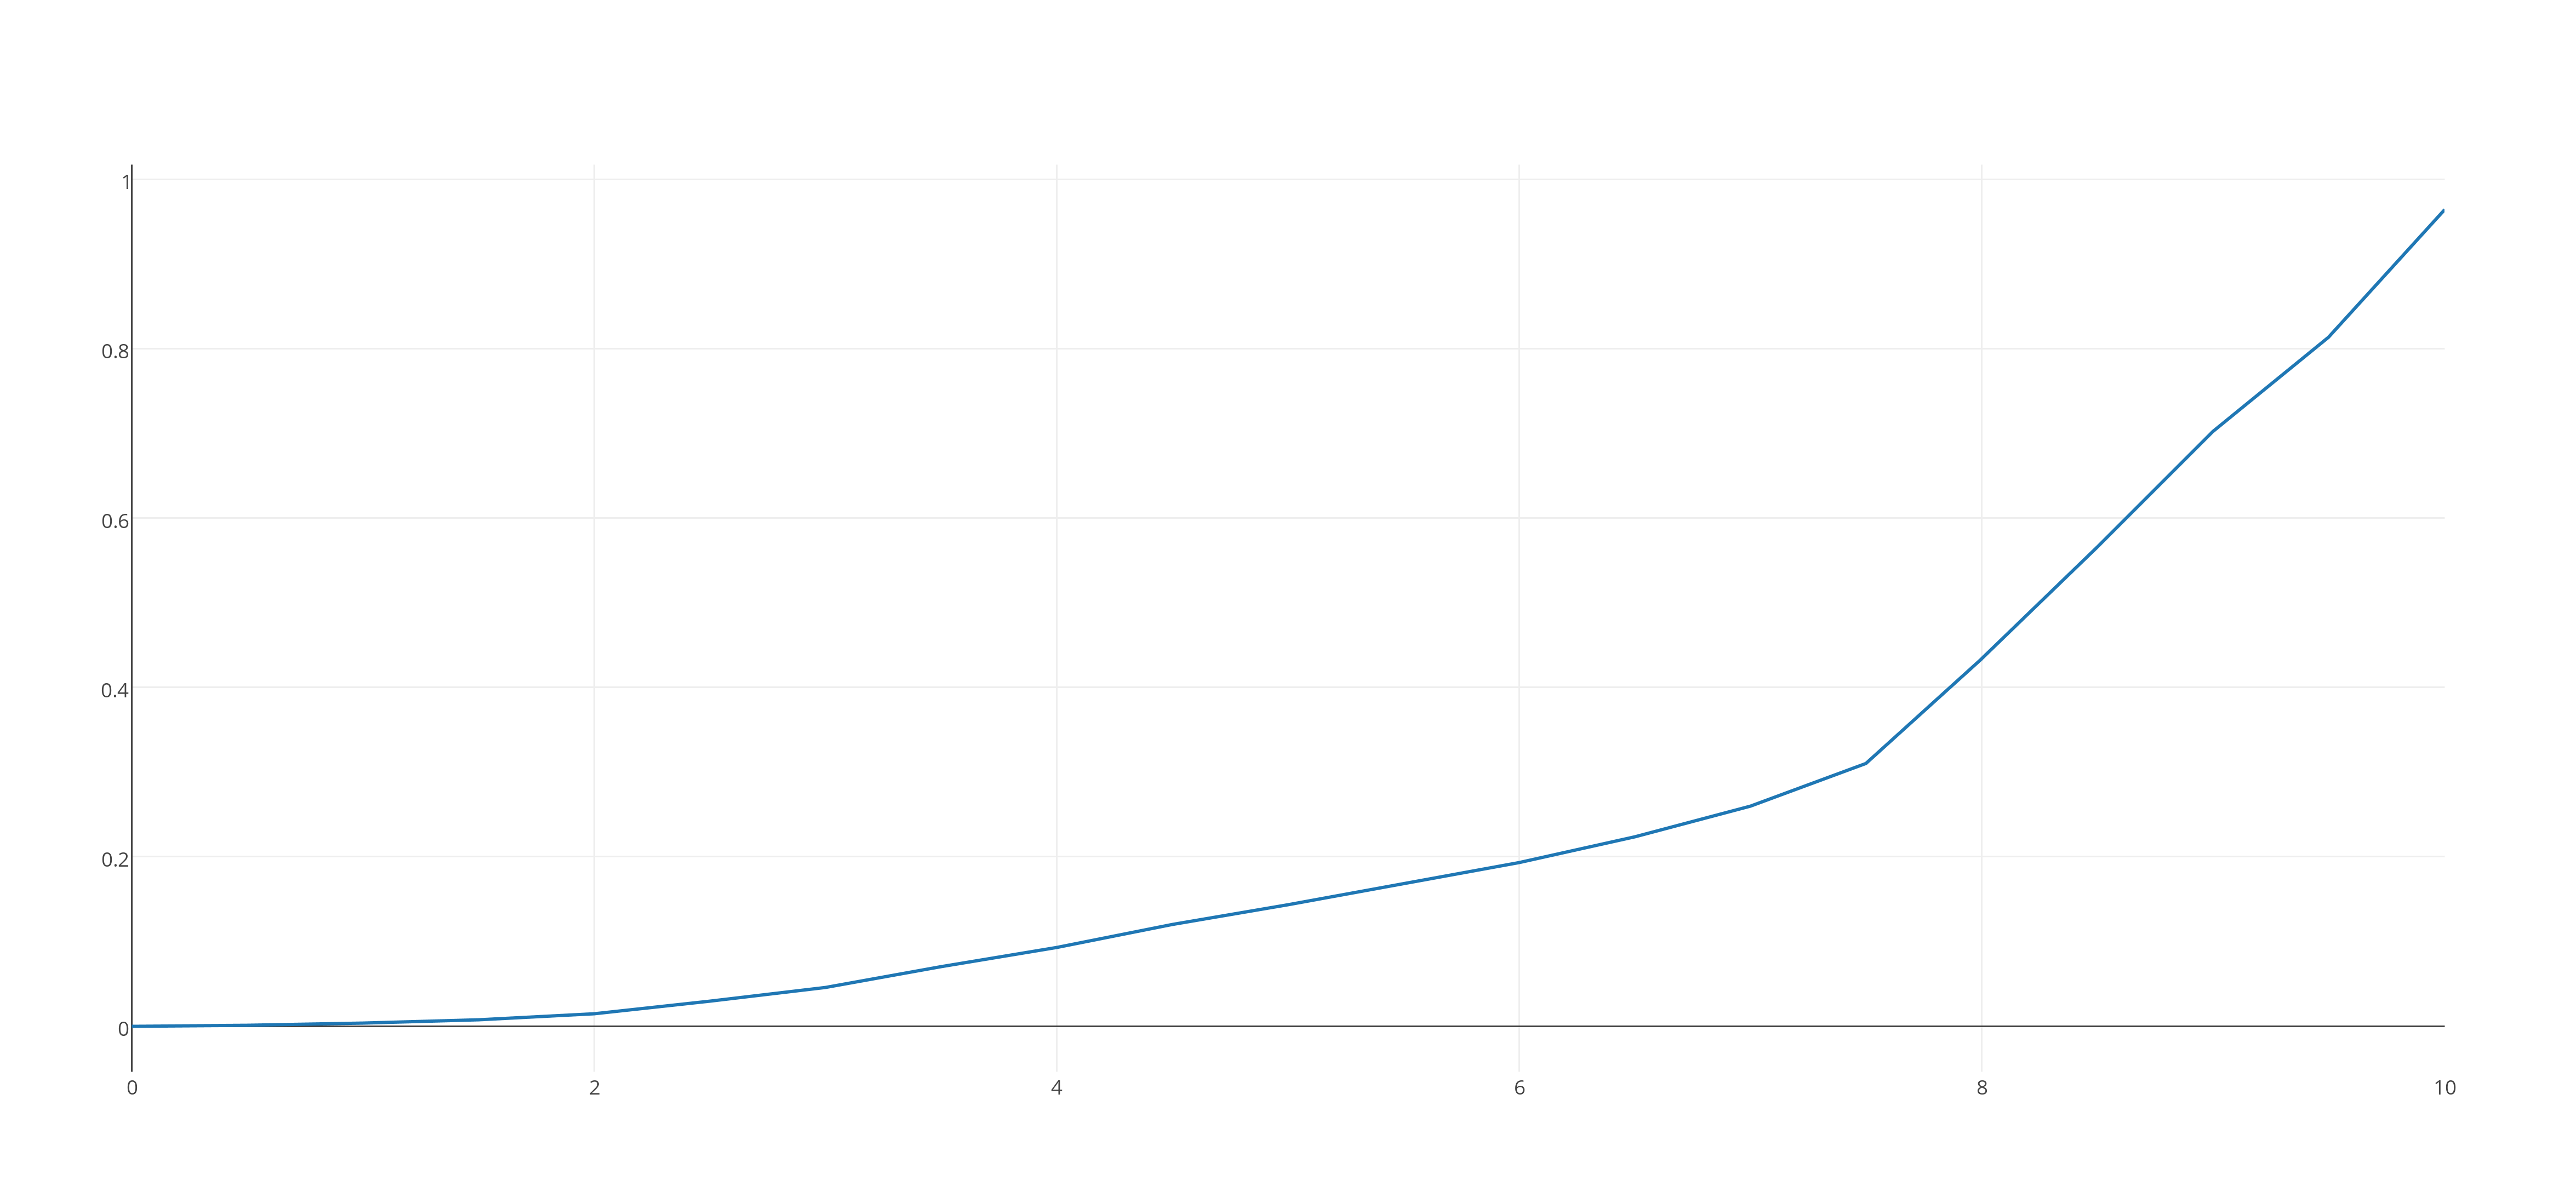
\includegraphics[width=0.5\textwidth, scale=0.5]{plot.png}
\vspace{1ex}
\hrule
\caption{Gemiddelde spanning per positie.}
\label{fig:measurings}
\end{figure}

Om de gemeten spanning om te zetten naar een potentiowaarde, hebben wij gebruik gemaakt van Wolfram Alpha om een geschikte fit te vinden. Om een zo nauwkeurig mogelijke vertaling te krijgen, maken wij tot een spanning van 0.165 (potentiowaarde 5.5) gebruik van een least-squares fit om een formule te vinden. Wanneer de spanning hoger is dan 0.165, wordt een exponential fit gebruikt.\\
Tot een spanning van 0.l65 wordt de volgende formule gebruikt, waarbij x de potentiowaarde is:
\begin{equation}
    spanning = 0.00599767 \cdot x^2 - 0.000904196 \cdot x - 0.00289697
\end{equation}
Boven een meting van 0.165 maken wij gebruik van de volgende exponentiele functie, waarbij eveneens x de potentiowaarde is:
\begin{equation}
    spanning = 0.0158139 \cdot e^{0.41411 \cdot x}
\end{equation}

Het volgende code fragment (figuur \ref{code:determinePotentio}) zet de gemeten delerfactor om in de potentiowaarde. Hierbij is de functie abc\_getX een functie die met behulp van de abc-formule de waarde voor x berkend, waarbij geldt:\\
$0.00599767 \cdot x^2 - 0.000904196 \cdot x - 0.00289697 = input$

\begin{figure}
\begin{lstlisting}
float getRealPotentioValue(float input)
{
    // if input is less than 0.165, use abc-formula for calculating the potentio
    if (input < 0.165) {
        return abc_getX(input);
    }
    
    // 0.0158139 e^(0.41411 x)
    input = input / 0.0158139;
    input = log(input);
    input = input / 0.41411;
    return input;
}
\end{lstlisting}
\vspace{1ex}
\hrule
\caption{Code voor bepalen potentiowaarde}
\label{code:determinePotentio}
\end{figure}

De grafiek, inclusief fit door middel van bovenstaande formules, is te zien in figuur \ref{fig:fit}.
\vspace{1em}
\begin{figure}[!htbp]
\centering
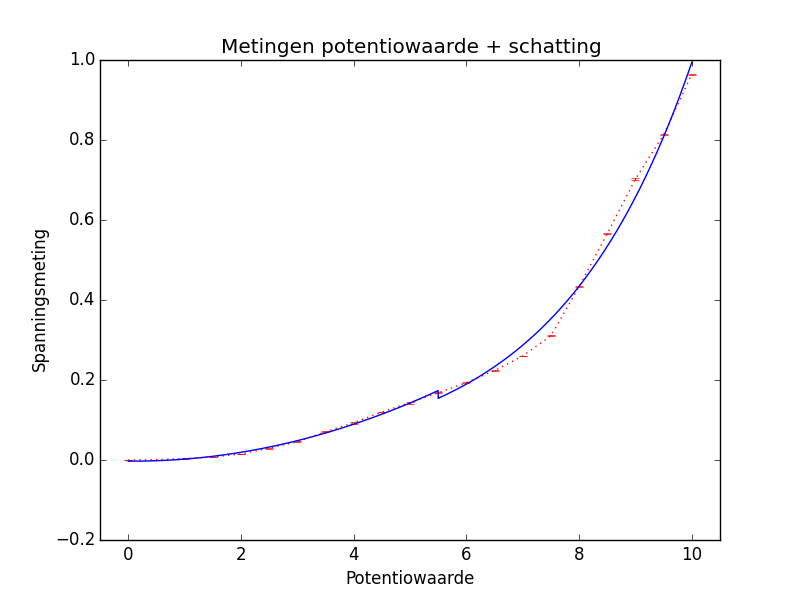
\includegraphics[width=0.8\textwidth, scale=0.8]{plot-with-estimate.png}
\vspace{1ex}
\hrule
\caption{Metingen potentiowaarden met schatting}
\label{fig:fit}
\end{figure}

Om de servomotor naar de juiste positie te verstellen, maken wij gebruik van de \texttt{forward()} of \texttt{backward()} methode. Dit hangt af van de huidige positie van de potentiometer. Wanneer de gewenste positie is bereikt, wordt de \texttt{stop()}-functie aangeroepen. Om te voorkomen dat de motor blijft draaien wanneer de minimum- of maximumwaarde is bereikt, hebben we een bovengrens van 6.5 seconden dat de motor kan draaien voor \'{e}\'{e}n aspositie regelingscommando.

Het volgende code-fragment (figuur \ref{code:gotoValue}) bevat de logica voor het instellen van een potentiowaarde. Er wordt in de richting van de gewenste waarde gedraaid, totdat deze waarde bereikt is of als er 6.5 seconden verstreken zijn.
\begin{figure}
\begin{lstlisting}
void goToValue(float destination) {
    float seconds = 0.0;
    if (destination < getCurrentValue()) {
        motor.backward();
        while(destination < getCurrentValue() && seconds < 6.5) {
            wait(0.1);
            seconds += 0.1;
        }
    } else {
        motor.forward();
        while(destination > getCurrentValue() && seconds < 6.5) {
            wait(0.1);
            seconds += 0.1;
        }
    }
    motor.stop();
}
\end{lstlisting}
\vspace{1ex}
\hrule
\caption{Code voor navigeren naar bepaalde potentiowaarde}
\label{code:gotoValue}
\end{figure}

\subsection{Android-mBed koppeling}
Een Android toestel wordt aangesloten op de USB-aansluiting van de mBed. Dit toestel gaat dienen als een \textit{slave}, d.w.z. een tussenstation om via de mBed commando's te sturen naar het servosysteem. Een tweede toestel, de \textit{master}, verbindt zich via een Bluetooth verbinding met de slave. Dit geeft het de mogelijkheid om draadloos de huidige weerstand op te vragen en via een Android-app met een draaiknop deze weerstand te wijzigen. Een android apparaat kan met verschillende slaves verbonden zijn, die via een menu kunnen worden geselecteerd. Op deze manier kunnen tegelijkertijd meerdere servosystemen worden bestuurd. Een slave die rechtsstreeks verbonden is aan een mBed heeft ook de mogelijkheid zelf commando's sturen naar het servosysteem.

%----------------------------------------------------------------------------------------
%	RESULTATEN
%----------------------------------------------------------------------------------------

%\section{Resultaten}

%----------------------------------------------------------------------------------------
%	DISCUSSIE
%----------------------------------------------------------------------------------------

\section{Discussie}
Het bepalen van de huidige potentiowaarde heeft enige problemen opgeleverd. In eerste instantie is een meting van het spanningssignaal gedaan voor elke halve potentiowaarde (0, 0.5, 1 .. 9.5, 10). Hier hebben wij een exponential fit op losgelaten. Dit leverde een potentiowaade die afwijkingen van potentiowaarde vertoonde van ruim 1. In een later stadia hebben wij besloten een betere bepaling te doen door middel van meerdere formules. Aangezien lage potentiowaarden zeer kleine verschillen tonen en de hogere waarden meer exponentiele verschillen, hebben wij besloten de lagere waarden met een least-squares fit te bepalen en de hogere waarden met een exponential fit. Uit een paar tests is gebleken dat de potentiowaarde het minst afwijking toonde als we de grens stelden op een spanningswaarde van 0.165.\\
Zoals in figuur \ref{fig:fit} te zien is, loopt de curve niet geheel gelijk aan de gemeten waarden.

De geschreven mBed code heeft voor het instellen van een potentiowaarde een tijdslimiet van 6.5 seconden. Als na 6.5 seconden de gewenste waarde nog niet bereikt is, wordt het draaien gestopt. In theorie werkt deze methode, maar door de implementatie van de draaiknop in de Android applicatie werkt het niet als gewenst. In de Android applicatie worden tijdens het draaien van de knop tussentijds meerdere requests naar de mBed gestuurd om de waarde aan te passen. Deze requests worden niet gebundeld, dus nadat het tijdslimiet van de request is verstreken, gaat hetzelfde tijdslimiet in voor de volgende requests. Hierdoor stopt de motor niet na de 6.5 seconden, zoals aanvankelijk verwacht wordt.

%\subsection{Implicaties en aanbevelingen}

%\subsection{Conclusie}

%----------------------------------------------------------------------------------------
%	REFERENTIES
%----------------------------------------------------------------------------------------
%Meer informatie hierover volgt in blok 5 van jaar 1.

\bibliographystyle{acm}

%----------------------------------------------------------------------------------------
%	BIJLAGEN
%----------------------------------------------------------------------------------------

%\section{Bijlage A}
%\section{Bijlage B}
%\section{Bijlage C}

\end{document}